\section{General relativity}

The need for a complete theory of gravity became apparent in the 19th century. Astronomical observations yielded data that violated the predictions of Newtonian gravity, among them mercury's perihelion shift\cite{1859AnPar...5....1L}, light deflection by the sun \cite{1920RSPTA.220..291D}, gravitational redshift in Sirius B \cite{2010JHA....41...41H}, and others. So far, Einstein's general relativity(GR) has proven accurate in describing these phenomena. In particular, as far as this research is concerned, it describes well the evolution and structure of the most compact objects in the universe: black holes and neutron stars, as well as binary systems that contain them.

GR has predicted that binary systems of compact objects lose radial separation due to significant emission of gravitational radiation. Such effects have been frequently observed in BNS systems by Hulse and Taylor \cite{Weisberg:1981mt} and LIGO\cite{LIGOScientific:2017vwq}, BBH by LIGO and Virgo \cite{LIGOScientific:2016aoc}, and NSBH by LIGO Virgo and KAGRA\cite{LIGOScientific:2021qlt}. Unfortunately, the two-body problem in GR has no analytical solution. Such systems and their gravitational waves must be studied by approximate and semi-analytical methods in their premerger stage or by numerical methods if one intends to study the complete evolution of the inspiral-merger-postmerger system\cite{Dietrich:2018phi}.

Although Einstein's general relativity is a broad theory with relevant consequences in several areas of astrophysics, the following section intends to make a simple introduction to the field equations, motivated by several sources such as the books by Inverno\cite{inverno}, Wald\cite{Wald:1984rg}, and Carroll\cite{carroll-notes}. Later it develops in a detailed way relativistic aspects of the physics of stars in hydrostatic equilibrium and gravitational waves, following in general lines, what is presented in the books of Weinberg\cite{Weinberg:1972kfs} and Hartle\cite{Hartle:2021pel}.



\subsection{Einstein's field equations}

After revolutionizing physics with the theory of special relativity in 1905 \cite{Einstein:1905}, Einstein took a few more years to elaborate a more general theory that could intrinsically include gravity in spacetime's geometry \cite{Einstein:1915ca}.

Various physical ideas and principles led Einstein to derive his field equations. In particular, Mach's principle \cite{mach1919science, 1995mpfn.conf.....B} and the equivalence principle largely influenced his theory. The geometry of spacetime, being responsible for the inertial motion of bodies and the mass/energy distribution of the universe contributing to that inertia, led Einstein to a set of tensor field equations relating the spacetime metric and its derivatives to the energy-momentum tensor of matter and fields living in it. However, other methods have been used to obtain the field equations, such as Hilbert \cite{Hilbert:1915tx} and Lovelock \cite{Lovelock:1971yv}. 

In 3+1 dimensions, Einstein's field equations are a set of 10 independent, second-order, coupled, nonlinear partial differential equations over the spacetime metric $g_{\mu \nu}$, that can be written in two compact forms



\begin{equation}\label{EFE}
G_{\mu\nu}  =  \frac{8\pi G}{c^4} \cdot T_{\mu\nu},
\end{equation}

\begin{equation}\label{EFE-ricci}
R_{\mu\nu}  =  \frac{8\pi G}{c^4} \cdot (T_{\mu\nu} - \frac{1}{2} g_{\mu\nu} T), 
\end{equation}

Where G and c are the gravitational constant and the speed of light in vaccuum. 

The left hand side of the equations is composed by the Einstein tensor $G_{\mu\nu}$, which is a combination of $R_{\mu\nu}$, $R$ called Ricci tensor, Ricci scalar. Definitions are listed below to help unveil that equations \ref{EFE} and \ref{EFE-ricci} are in fact, partial diferential equations for the metric components $g_{\mu\nu}$:


\begin{itemize}
\item Christoffel symbols

\begin{equation}\label{christoffel}
\Gamma^{\alpha}_{\beta \gamma} = \frac{1}{2} g^{\alpha \delta}(\partial_{\beta} g_{\delta \gamma} + \partial_{\gamma} g_{\delta \beta} - \partial_{\delta} g_{\beta \gamma})
\end{equation}

\begin{equation}
\Gamma^{\alpha}_{\beta \gamma} = \Gamma^{\alpha}_{\gamma \beta}
\end{equation}


\item The Riemann tensor, Ricci tensor and Ricci scalar 
\begin{equation}\label{riemann}
R^{\alpha}_{\mu\gamma \delta} = \partial_{\gamma} \Gamma^{\alpha}_{\mu \delta} - \partial_{\delta} \Gamma^{\alpha}_{\gamma \mu} +  \Gamma^{\alpha}_{\gamma \lambda} \Gamma^{\lambda}_{\delta \mu} - \Gamma^{\alpha}_{\delta \lambda} \Gamma^{\lambda}_{\gamma \mu}
\end{equation}

\begin{equation}
R_{\alpha \beta}= R^{\delta}_{\alpha \delta \beta}
\end{equation}

\begin{equation}
R = g^{\alpha \beta}R_{\alpha \beta}
\end{equation}

\item The Einstein tensor, i.e. the trace reversed Ricci tensor

\begin{equation}
G_{\mu\nu} = R_{\mu\nu} - \frac{1}{2} g_{\mu\nu} R
\end{equation}


\end{itemize}


The process of solving equations\ref{EFE} to obtain the spacetime metric, and solving the geodesic equations 

\begin{equation}\label{par-trans}
u^{\delta} \nabla_{\delta } u^{\alpha } = 
0 \rightarrow \frac{d^2 x^{\alpha}}{d\tau^2} = - \Gamma^{\alpha}_{\nu\mu} \frac{dx^{\nu}}{d\tau} \frac{dx^{\mu}}{d\tau},
\end{equation}

is the relativistic analogous to what in newtonian case would be solving the Poisson equation\ref{poisson} to obtain the potential $\phi$ and using Newton's second law to obtaining particle trayectories on the gravitational field. Where  $\nabla_{\delta}$ are the components of a unique covariant derivative operator acting on the particle's 4-velocity $u^{\alpha}$(see Wald\cite[chapter X]{Wald:1984rg}). 

In addition, tidal interactions between particles induced by the curvature of spacetime can be measured by the geodesic deviation equation(see Hartle \cite[chapter X]{Hartle:2021pel}). The relativistic analogous of equation\ref{tidal0}, encodes the geometry of spacetime via the Riemann tensor components $R^{\alpha}_{\;\; \tau \mu \tau}$

\begin{equation}\label{tidal1}
\frac{d \xi^{\alpha}}{d\tau} = - R^{\alpha}_{\;\; \tau \mu \tau} \cdot \xi^{\mu}
\end{equation} 


On the other hand, the right hand side of the equations \ref{EFE} contains information about the fluids, particles and fields present in spacetime. Spacetime and stress-energy are coupled, such that physically relevant solutions to the field equations must satisfy $\nabla_{\mu} T^{\mu\nu} = 0$, since the second Bianchi identity leads to zero divergence of the Einstein tensor $\nabla_{\mu}G^{\mu\nu} = 0$ (see \cite{inverno, Wald:1984rg, Weinberg:1972kfs}).

Some energy-momentum tensors inherited from special relativity have given rise to analytical solutions of the einstein equations such as the TOV equation \cite{PhysRev.55.374} and the Reinser-Nordstrom solution \cite{https://doi.org/10.1002/andp.19163550905}. In a local inertial frame, the stress-energy tensor for perfect fluids, and the Faraday tensor can be written as


\begin{equation}\label{PF}
T^{\mu \nu} = 
\begin{pmatrix}
\rho \cdot c^2&0&0&0 \\
0&-p&0&0 \\
0&0&-p&0 \\
0&0&0&-p\\
\end{pmatrix} \;\; ,
\end{equation}

\begin{equation}
F_{\mu \nu} = 
\begin{pmatrix}
0&\frac{E_x}{c}&\frac{E_y}{c}&\frac{E_z}{c} \\
-\frac{E_x}{c} &0   &B_z  &B_y \\
-\frac{E_y}{c} &-B_z&0    &B_x \\
-\frac{E_z}{c} &-B_y&-B_x &0\\
\end{pmatrix} \;\;,
\end{equation}


Where $\rho$ is the rest mass density, p is the pressure, $E_i$ is the ith component od the electric field, $B_j$ is the jth component of a magnetic field and c is the speed of ligth in vaccum. Both have been relevant in theoretical applications of GR like idealized neutron stars or quark-gluon plasmas \cite{Nagle_2011}, and charged black holes respectively \cite{PhysRevD.13.2713}.

Due to their nonlinear and coupled character, analytical solutions to the Einstein equations are challenging to find. In particular to study systems like CBCs numerical simulations have been employed to study the entire binary evolution since the 2000s \cite{Shibata:1999hn,Shibata:1999wm,Shibata:2019wef} and  approximate methods such as post-Newtonian expansions to study their inspiral phases(see Creighton et.al \cite[chapter X]{Creighton:2011zz}). 

Although this thesis focuses on doing data analysis with gravitational waves extracted from fully relativistic numerical simulations \cite{Bishop:2016lgv}, physical consequences like the existence of a maximum mass for a static star and the quadrupolar nature of gravitational waves are key to understand the results of such simulations and their applications in gravitational wave astronomy. For this reason following subsections will treat in detail the Tolman-Oppenheimer-Volkoff equation for relativistic star in hydrostatic equilibrium and  the first-order approximation that led Einstein to predict gravitational waves in 1916.



\subsection{Spherically symmetric stars and the TOV equation}\label{codeon}

To date, GR predictions have coicided with observations of compact objects like neutron stars(NSs) and black holes(BHs). The internal structure of NSs have been acurately studied using a generalized version of equation \ref{press.grad}, which together with the matter model encoded in an equation of state, can tell about the star's properties like the tidal deformability(see equation \ref{Tid}), mass and radius, as well as the pressure and density profiles. 

The EOS for NSs is currently not well constrained. Observations of known pulsars and gravitational wave events like GW170817 are currently being used to improve existing constraints on the EOS of supranuclear matter. The following is going to be a detailed derivation of the equation for stars in hydrostatic equilibrium in general relativity following Weinberg's book\cite{Weinberg:1972kfs}. Mass-radius diagrams will not be computed since they require numerical integration even for simple EOSs like the polytropic one(see equation \ref{EOS0}). However, the mass-radius relations for several EOSs used in BNS simulations will be shown, to depict their difference with their Newtonian analogue, and emphasize their main feature: the prediction of a maximum amount of mass each EOS can support(see figure \ref{equations of state and tidal deformability}).

Let us start with a static and spherically symmetric spacetime metric

\begin{equation}\label{metric}
ds^2 = B(r) dt \otimes dt - A(r) dr \otimes dr - r^2 (d\theta \otimes d\theta + \sin^2 \theta \; d\phi \otimes d\phi)
\end{equation}

Its non-vanishing Ricci tensor components  can be written in terms of the functions $A(r)$, $B(r)$(see \cite{Weinberg:1972kfs}). Plugging them in the left hand side of equations \ref{EFE-ricci} and assuming the stress-energy tensor of a perfect fluid \ref{PF} on the right side gives

\begin{equation}\label{E1}
R_{rr} = \frac{B''}{2B} - \frac{B'}{4B} \left( \frac{A'}{A}+\frac{B'}{B} \right) - \frac{A'}{rA} = -4\pi G(\rho-P) A
\end{equation}

\begin{equation}\label{E2}
R_{\theta \theta}  = -1 + \frac{r}{2A} \left( -\frac{A'}{A} + \frac{B'}{B} \right) + \frac{1}{A} = -4\pi G(\rho - P) r^2
\end{equation}

\begin{equation}\label{E3}
R_{tt} = - \frac{B''}{2A} + \frac{B'}{4A} \left( \frac{A'}{A}+\frac{B'}{B} \right) - \frac{B'}{rA} = - 4\pi G (\rho + 3P) B
\end{equation}

Now, the divergencelessness condition for the energy momentum tensor will used to obtain an expression for the metric coefficient $B(r)$ and its first derivative $B'$. Later, the components of the Ricci tensor will be combined in a convinient way to do the same for $A(r)$ and its first derivative $A'$. 

The stress-energy tensor for a perfect fluid \ref{PF} can be written in components as

\begin{equation}
T^{\mu \nu} = (\rho + P) u^\mu u^\nu + P g^{\mu \nu}
\end{equation}

After plugging it in the covariant divergencelessness condition 

\begin{equation}
0 = \nabla_\nu T^{\mu \nu}
\end{equation}

\begin{equation}
0 =  \partial_\nu T^{\mu \nu} + \gamma^\mu_{\nu \delta} T^{\delta \nu} + \gamma^\nu_{\nu \delta} T^{\mu \delta}
\end{equation}

Becomes the following lenghty expression

\begin{equation}
\begin{matrix}
0 = (\partial_\nu P) g^{\mu \nu} + P \partial_\nu g^{\mu \nu} +\partial_\nu \left[ (P+\rho) u^\mu u^\nu \right]+ \\ \Gamma^\nu_{\nu \delta}(P g^{\mu \delta} + (\rho+P)u^\mu u^\delta ) + P \Gamma^\mu_{\nu \delta} g^{\nu \delta} +\Gamma^\mu_{\nu \delta} (\rho+ P) u^\delta u^\nu.
\end{matrix}
\end{equation}

\begin{equation}
0 = (\partial_\nu P) g^{\mu \nu} + \Gamma^\nu_{\nu \delta}(P g^{\mu \delta} + (\rho+P)u^\mu u^\delta ) + \partial_\nu \left[ (P+\rho) u^\mu u^\nu \right]+ \Gamma^\mu_{\nu \delta} (\rho+ P) u^\delta u^\nu.
\end{equation}

\begin{equation}\label{glk}
\begin{matrix}
0 = (\partial_\nu P) g^{\mu \nu} + g^{-\frac{1}{2}}\partial_\nu(g^{\frac{1}{2}})  (P g^{\mu \delta} + (\rho+P)u^\mu u^\delta ) + \partial_\nu \left[ (P+\rho) u^\mu u^\nu \right]+ \Gamma^\mu_{\nu \delta} (\rho+ P) u^\delta u^\nu.
\end{matrix}
\end{equation}

Where we have used the identity $\Gamma^\mu_{\mu \nu}=g^{-\frac{1}{2}}\partial_\nu(g^{\frac{1}{2}})$(see Inverno \cite[chapter 7]{inverno}) and the compatibility of the metric to eliminate some terms. 

Further, we evaluate energy-momentum conservation in the rest frame of the fluid, where its 4-velocity takes the form $u=(\sqrt{g_{00}},0,0,0,0)$.  In such a frame, equation \ref{glk} takes a much simpler form since only the timelike components of the 4-velocity contribute, and the pressure and density profiles will not depend on time. The relevant Christoffel symbols also take a simple form, and the metric trace vanishes after differentiation. 

\begin{equation}
0 = (\partial_\nu P) g^{\mu \nu} + \Gamma^\mu_{00} (\rho+ P) (u^0)^2 + \partial_0 \left[ (P+\rho) u^\mu u^0 \right]
\end{equation}

\begin{equation}
0 = (\partial_\nu P) g^{\mu \nu} + \left(-\frac{1}{2}g^{\mu \nu} \partial_\nu g_{00} \right) (\rho+ P) (u^0)^2 
\end{equation}

\begin{equation}
-(\partial_\nu P) g^{\mu \nu} = (\rho+ P) g^{\mu \nu} \partial_\nu \ln{(-g_{00})^{\frac{1}{2}}}
\end{equation}

\begin{equation}\label{ener.cond0}
-\partial_\lambda P  = (\rho+ P)  \partial_\lambda \ln{(-g_{00})^{\frac{1}{2}}}
\end{equation}

Taking $g_{00} = -B(r)$, equation \ref{ener.cond0} becomes an equation for B and its first derivative

\begin{equation}\label{B'/B}
\frac{-2P'}{(P+\rho)} = \frac{B'}{B}
\end{equation}


To get an equation for $A$ and $\frac{A'}{A}$, we use the following combination of the Ricci tensor components:

\begin{equation}
\frac{R_{rr}}{2A} +\frac{R_{\theta \theta}}{r^2} + \frac{R_{tt}}{2B} = -\frac{A'}{rA^2} - \frac{1}{r^2} + \frac{1}{A r^2} = -8\pi G \rho
\end{equation}

\begin{equation}
\frac{1}{r^2} \left[ \left(\frac{r}{A} \right)' - 1 \right] = -8\pi G \rho
\end{equation}

\begin{equation}
 \left(\frac{r}{A}\right)' = 1 - 8\pi G r^2 \rho
\end{equation}

\begin{equation}
\left(\frac{r}{A}\right) = r - 2G \int_0^r dr'4\pi  r'^2 \rho(r')
\end{equation}

\begin{equation}
\left(\frac{r}{A}\right) = r - 2G M(r)
\end{equation}

Where $M(r)$ is given by

\begin{equation}\label{oreijf}
M(r):= \int_0^r dr'4\pi  r'^2 \rho(r')
\end{equation}


So that, we finally arrive at 

\begin{equation}\label{A}
A = \left[ 1 - \frac{2G M(r)}{r} \right]^{-1}
\end{equation}

\begin{equation}\label{A'/A}
\frac{A'}{A} = \frac{2G(M/r)'}{1-\frac{2GM(r)}{r}}
\end{equation}


Inserting equations \ref{A},\ref{A'/A} and \ref{B'/B}, in  $R_{\theta \theta}$ we get an equation for the pressure gradient in terms of $M(r)$, $P(r)$ and $\rho(r)$

\begin{equation}
-1 + \frac{r}{2A} \left( -\frac{A'}{A} + \frac{B'}{B} \right) + \frac{1}{A} = -4\pi G(\rho - P) r^2
\end{equation}

\begin{equation}
-1 + Gr \left( \frac{M}{r}\right)' - \left[ 1-\frac{rP'}{(P+\rho)} \right] = -4\pi G(\rho - P) r^2
\end{equation}

\begin{equation}
-1 + \frac{GM}{r^2} -\frac{GrM'}{r} - \left[ 1-\frac{rP'}{(P+\rho)} \right] = -4\pi G(\rho - P) r^2
\end{equation}

\begin{equation}
-GM' - \left[ 1 - \frac{2GM}{r}\right] - \left[ 1-\frac{rP'}{(P+\rho)} \right]\left(  1 - \frac{2GM}{r} \right) = -4\pi G(\rho - P) r^2
\end{equation}

\begin{equation}
-1 + \left[ 1-\frac{rP'}{(P+\rho)} \right]\left(  1 - \frac{2GM}{r} \right)+\frac{GM}{r} - 4\pi G r^2 \rho(r) = -4\pi G(\rho - P) r^2
\end{equation}

\begin{equation}
- \left( \frac{rP'}{(P+\rho)}\right)\left(  1 - \frac{2GM}{r} \right) - \frac{GM}{r} = + 4\pi G P r^2
\end{equation}

\begin{equation}
- \left( \frac{rP'}{(P+\rho)}\right)\left(  1 - \frac{2GM}{r} \right) = \frac{G}{r} \left( M + 4\pi r^3 P \right)
\end{equation}

\begin{equation}
- \left( \frac{P'}{(P+\rho)}\right) = \frac{G}{r^2} \frac{\left( M + 4\pi r^3 P \right)}{\left(  1 - \frac{2GM}{r} \right)}
\end{equation}

\begin{equation}
- P' = \frac{G}{r^2} \frac{\left( M + 4\pi r^3 P \right)}{\left(  1 - \frac{2GM}{r} \right)} (P+\rho)
\end{equation}

\begin{equation}\label{TOV2}
- P' = \frac{G}{r^2} \frac{\left( M + 4\pi r^3 \frac{P}{c^2} \right)}{\left(  1 - \frac{2GM}{r c^2} \right)} \left( \frac{P}{c^2}+\rho \right)
\end{equation}

The equation \ref{TOV2} is called Tolman-Oppenheimer-Volkoff equation(TOV). Notice how it reduces to the Newtonian equation \ref{press.grad} when taking the limits $c\rightarrow \infty$ and $GM/c^2 <<1$. The system of equations \ref{TOV2}, \ref{oreijf} must be completed by an EOS $P(\rho)$, and solved by using numerical methods.

The following figure shows NS properties for the EOSs present in the CoRe catalog for BNS waveforms \cite{Dietrich:2018phi}. One of the most important features of GR is the prediction of a maximum in every curve of the mass-radius relation(left panel). It is called the maximum TOV mass, and serves as a reference for the amount of matter an EOS can support. Notice the almost EOSs independent relation between the compactness parameter and the tidal deformability(see equation \ref{Tid}) of a static star(right panel). 

\begin{figure}[hbt!]
\begin{center}
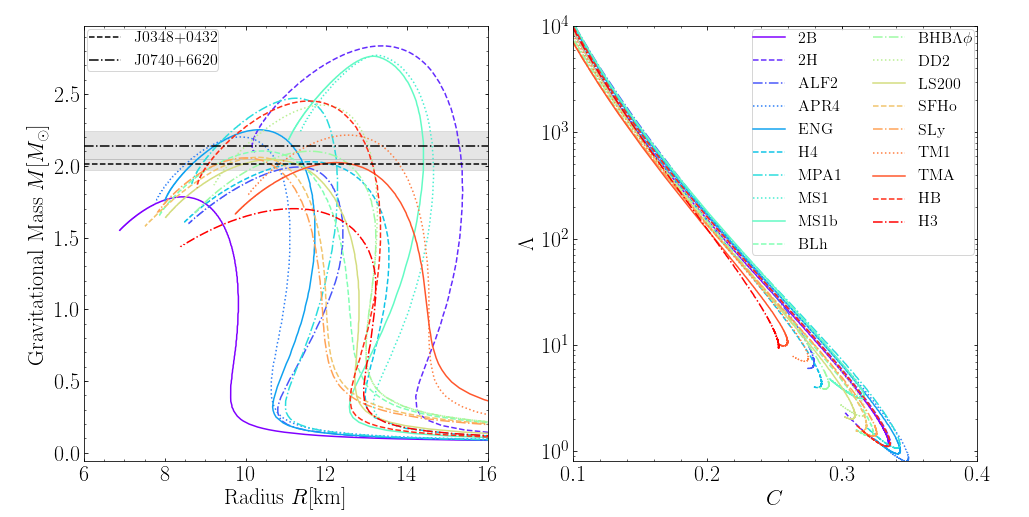
\includegraphics[width=0.8\textwidth, angle=0]{images/EOS_TOV.png}
\captionsetup{width=.8\textwidth}
\caption{NS properties for the CoRe EOS database}
\caption*{This image was taken from \cite{EOSDB}. It shows the mass-radius relations(left) for the CoRe EOS database \cite{Dietrich:2018phi}, and their compactness-tidal deformability relations(right).}
\label{equations of state and tidal deformability}
\end{center}
\end{figure}

\FloatBarrier

Recent studies have investigated the existence of a threshold mass for realistic neutron stars produced by BNS mergers \cite{Kashyap_2022}. Such scenarios may produce either prompt collapse to a BH, or a differentially rotating fluid that can delay the collapse for a few milliseconds while emitting gravitational waves, and have been classified according to the ratio

\begin{equation}\label{delta}
\delta=\frac{M_g}{M_{TOV}}
\end{equation} 

Where $M_g$ is the total gravitational mass, and $M_{TOV}$ is the maximum TOV mass.




\subsection{Linearized theory and gravitational radiation}\label{GW}

Even though Einstein himself was sceptical about someone finding  exact solutions to \ref{EFE}, he came up with the first approximate solution of his equations in 1916 \cite{Einstein:1916cc}. The equations he found admitted wave-like solutions that would produce the following effects on a ring of particles via tidal accelerations given by equation \ref{tidal1}


\begin{figure}[hbt!]
\begin{center}
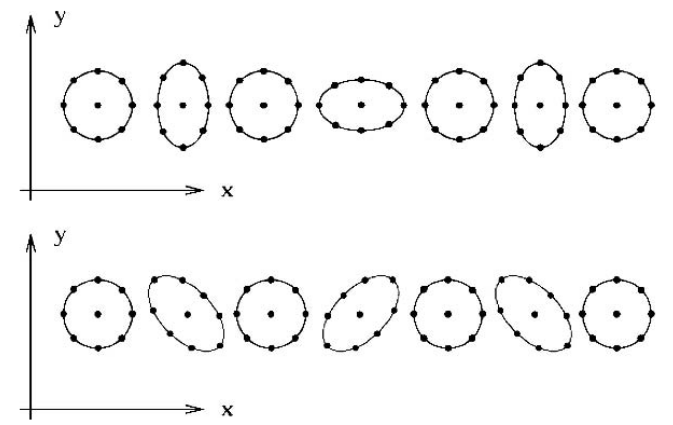
\includegraphics[width=0.6\textwidth, angle=0]{images/particle-ring.png}
\captionsetup{width=0.8\textwidth}
\caption{Gravitational waves interacting with a ring of test masses}
\caption*{This image was taken from \cite{carroll-notes}.  It shows The effects of the two gravitational waves polarization on a ring of test masses.The phases shown are 0, $\frac{\pi}{2}$, $\pi$, $\frac{3\pi}{2}$, and $2\pi$ respectively.
}
\label{GW passing through a ring of test masses}
\end{center}
\end{figure}

\FloatBarrier

The following derivation is carried out to show the consequences of linearizing Einstein Field equations. To do so, we follow the books by Hartle \cite{Hartle:2021pel}, Creighton et.al. \cite{Creighton:2011zz} and Schutz \cite{Schutz:1985jx}. 

Let us begin by expanding the metric $g$ to first order around the background Minkowski metric 

\begin{equation}\label{metric}
g_{\mu \nu} =  \eta_{\mu \nu} + h_{\mu \nu}.
\end{equation}

Where the components of $h_{\mu \nu}$ are said to be a small, i.e. $h_{\mu \nu}<<1$ as compared to Minkowski metric $\eta_{\mu \nu}$  in an coordinate system where $\eta$ components are $diag(-1,1,1,1)$. Such first-order approximation will allow the Christoffel symbols to be written in terms of the metric perturbation and its derivatives

\begin{equation}\label{cris}
\Gamma^{\alpha}_{\beta \gamma} = \frac{1}{2} \eta^{\alpha \delta}(\partial_{\beta} h_{\delta \gamma} + \partial_{\gamma} h_{\delta \beta} - \partial_{\delta} h_{\beta \gamma}),
\end{equation}

In addition, the Riemann tensor, the Ricci tensor and the Ricci scalar become much simpler

\begin{equation}
R^{\alpha}_{\beta \mu\nu} = -\frac{1}{2} \eta^{\alpha \lambda} [ \partial^2_{\lambda \mu} h_{\beta \nu} + \partial^2_{\beta \nu} h_{\lambda \mu} - \partial^2_{\lambda \nu} h_{\beta \mu} - \partial^2_{\beta \mu} h_{\lambda \nu}],
\end{equation}

\begin{equation}
R_{\beta \nu} = -\frac{1}{2} [ \Box h_{\beta \nu} + \partial_{\beta}\partial_{\nu} h - \partial_{\nu} \partial^{\gamma} h_{\beta \gamma} - \partial_{\beta} \partial^{\lambda} h_{\lambda \nu} ],
\end{equation}

\begin{equation}\label{mcieuf}
R_{\beta \nu} = -\frac{1}{2} [ \Box h_{\beta \nu} + \partial_{\beta}\partial_{\nu} h - \partial_{\nu} \partial^{\gamma} h_{\beta \gamma} - \partial_{\beta} \partial^{\lambda} h_{\lambda \nu} ],
\end{equation}


\begin{equation}\label{cxndown}
R = -\frac{1}{2} \Box h + \partial^{\alpha}\partial^{\beta} h_{\alpha \beta}.
\end{equation}

Motivated by equation \ref{EFE},  which uses the trace reversed Ricci tensor $G_{\mu \nu}= R_{\mu\nu}-\frac{1}{2} g_{\mu\nu} R$ in the left hand side, one can also use a reversed version of $h$


\begin{equation}
\bar{h}_{\mu\nu} = h_{\mu\nu}-\frac{1}{2} \eta_{\mu\nu} h
\end{equation}

\begin{equation}\label{xeiufbc}
R_{\beta \nu} = -\frac{1}{2} [ \Box( \bar{h}_{\beta \nu}-\frac{1}{2} \eta_{\beta \nu} \bar{h} ) - \partial_{\nu} \partial^{\gamma} \bar{h}_{\beta \gamma} - \partial_{\beta} \partial^{\lambda} \bar{h}_{\lambda \nu} ]
\end{equation}

\begin{equation}\label{cncob}
R = -\frac{1}{2} \Box \bar{h} + \partial^{\alpha}\partial^{\beta} \bar{h}_{\alpha \beta}
\end{equation}


Now, we can use equations \ref{mcieuf}, \ref{cxndown} to write down equations \ref{EFE} and  \ref{xeiufbc}, \ref{cncob} to write down equations \ref{EFE-ricci} to first oder as second order partial differential equations for $\bar{h}_{\mu \nu}$ and $h_{\mu\nu}$ respectively

\begin{equation}\label{hbar}
G^{(1)}_{\mu\nu} = \frac{8\pi G}{c^4} T^{(1)}_{\mu\nu} \rightarrow \bar{\mathcal{D}}^{\mu\nu}_{\alpha \beta} \bar{h}_{\mu\nu} = \frac{8\pi G}{c^4} T^{(1)}_{\mu\nu}
\end{equation}


\begin{equation}\label{h}
R^{(1)}_{\mu\nu} = \frac{8\pi G}{c^4}(T^{(1)}_{\mu\nu} - \frac{1}{2} \eta_{\mu\nu}T^{(1)}) \rightarrow \mathcal{D}^{\mu\nu}_{\alpha \beta} h_{\mu\nu} = \frac{8\pi G}{c^4}(T^{(1)}_{\mu\nu} - \frac{1}{2} \eta_{\mu\nu}T^{(1)})
\end{equation}


Where $\mathcal{D}$ and $\mathcal{\bar{D}}$ are the following second order differential operators:

\begin{equation}\label{D}
\mathcal{D}^{\mu\nu}_{\alpha \beta} = -\frac{1}{2}( \delta^{\mu}_{\alpha} \delta^{\nu}_{\beta} \Box + \eta^{\mu\nu}\partial_{\alpha}\partial_{\beta} - \delta^{\nu}_{\beta} \partial_{\alpha}\partial^{\mu} - \delta^{\nu}_{\alpha} \partial_{\beta}\partial^{\mu}),
\end{equation}

\begin{equation}\label{Dbar}
\bar{\mathcal{D}}^{\mu\nu}_{\alpha \beta} = -\frac{1}{2}( \delta^{\mu}_{\alpha} \delta^{\nu}_{\beta} \Box + \eta^{\alpha \beta}\partial^{\mu}\partial_{\nu} - \delta^{\nu}_{\beta} \partial_{\alpha}\partial^{\mu} - \delta^{\nu}_{\alpha} \partial_{\beta}\partial^{\mu}).
\end{equation}


It can be shown that equations \ref{h} and \ref{hbar} will determine the space-time perturbations $h$ or $\bar{h}$ up to redefinitions of the form

\begin{equation}\label{ondeoid}
h_{\mu\nu} \rightarrow  h^{'}_{\mu\nu} = h_{\mu\nu} + \partial_{\mu} \Lambda_{\nu} + \partial_{\nu} \Lambda_{\mu} 
\end{equation}


\begin{equation}\label{kcome}
\bar{h}_{\mu\nu} \rightarrow  \bar{h}^{'}_{\mu\nu} = \bar{h}_{\mu\nu} + \partial_{\mu} \Lambda_{\nu} + \partial_{\nu} \Lambda_{\mu} - \eta_{\mu\nu} \partial^{\delta} \Lambda_{\delta}
\end{equation}

Equations \ref{ondeoid} and \ref{kcome} represent the gauge freedom of general relativity comming from infinitesimal isometries of space-time(see Wald \cite[chapter X]{Wald:1984rg}). 

The redundancy caused by such freedom can be solved by imposing an additional condition. The following equation is called the de Donder gauge condition

\begin{equation}
g^{\mu\nu} \Gamma^{\lambda}_{\mu\nu} = 0
\end{equation}

Which is used to simplify the equations \ref{hbar} and \ref{h}. Recalling the Christoffel symbols \ref{cris}, it can be written ass follows  

\begin{equation}\label{doine}
\partial^{\mu} h_{\mu\nu} = \frac{1}{2} \partial_{\nu} h^{\delta}_{\delta}
\end{equation}

\textbf{Remark:} It can be shown that if a metric perturbation do not satisfy \ref{doine}, one can always perform the following transformation, to find a $\tilde{h}_{\mu\nu}$ that does(See Weinberg \cite[chapter 10]{Weinberg:1972kfs}):

\begin{equation}
\Box \Lambda_\nu = \partial^{\mu} h_{\mu\nu} - \frac{1}{2} \partial_{\nu} h^{\delta}_{\delta}
\end{equation} 

Inserting equation \ref{doine} in \ref{hbar} makes the operator \ref{D} become much simpler


\begin{equation}\label{waveeq}
\left( -\frac{1}{2} \delta_{\mu}^{\alpha} \delta_{\nu}^{\beta} \Box \right) h_{\alpha \beta} = \frac{8\pi G}{c^4} \cdot (T^{(1)}_{\mu\nu} - \frac{1}{2} \eta_{\mu\nu} T^{(1)}),
\end{equation}


\begin{equation}\label{dedonder1}
\Box h_{\mu\nu} = -\frac{16\pi G}{c^4} \cdot (T^{(1)}_{\mu\nu} - \frac{1}{2} \eta_{\mu\nu} T^{(1)})
\end{equation}

\begin{equation}\label{dedonder2}
\Box \bar{h}_{\mu\nu} = -\frac{16\pi G}{c^4} \cdot (T^{(1)}_{\mu\nu})
\end{equation}
 

Finally, both equations \ref{waveeq} and \ref{dedonder1} must be solved simultaneously, by either using numerical or analytical methods such as retarded Green's functions in the non-vacuum case. 


\subsection{GW polarizations: transverse traceless gauge}

In contrast to Newtonian gravity, solutions to the vacuum equations of linearized gravity are already interesting enough to be studied. The simplest oscillatory "Ansatz" admitted by the  d'Alembert operator $\Box$ has the form   

\begin{equation}\label{planew}
h_{\mu\nu} = A_{\mu\nu} e^{i k_{\delta} \cdot x^{\delta}},
\end{equation}

where $k = (w/c, \vec{k})$ is a 4-vector containing the direction of the wavefront in spacetime. Let us take equation \ref{waveeq} in vaccuum, i.e. $T^{(1)}_{\mu \nu} = 0$, and plug in the plane wave Ansatz

\begin{equation}
\Box h_{\alpha \beta} = \eta^{\mu \nu} \partial_{\mu} \partial_{\nu} \left( A_{\alpha \beta} e^{(i k_{\delta} x^{\delta})} \right) = 0 
\end{equation}

\begin{equation}
- k^\delta k_\delta h_{\alpha \beta} = 0 
\end{equation}

We find that $k$ is a lightlike 4-vector, and the dispersion relation of gravitational waves is 

\begin{equation}
h_{\alpha \beta} \neq 0, \;\; k^\delta k_\delta = 0
\end{equation}

\begin{equation}
(w/c)^2 - || \vec{k} ||^2 = 0
\end{equation}

It can be shown that the de Donder gauge leaves some gauge freedom remaining(see Hartle \cite[chapter X]{Hartle:2021pel}). For that reason, in the case of vacuum equations, the remaining gauge freedom can be fixed completely by choosing the following conditions

\begin{equation}\label{coindoi}
\begin{gathered}
h_{0i} = 0  \hspace{1cm} h_{00} = 0 \\
h = h^{\delta}_{\delta} = 0  \hspace{1cm} k^{i}h_{ij} = 0
\end{gathered}
\end{equation}

Which reduces the degrees of freedom of gravitational waves from 10 to 2. Let us see this for the case of a plane wave incoming from the z-direction. For such a wave, the 4-vector $k$ reads

\begin{equation}
k = (w/c, 0,0,k_z)
\end{equation}

Using the conditions \ref{coindoi} the metric perturbation takes the form 

\begin{equation}\label{met_pert}
h_{\mu \nu} \theta^\mu \otimes \theta^\nu = 
\begin{pmatrix}
0&0&0&0 \\
0&h_+ &h_\times &0 \\
0&h_\times &-h_+ &0 \\
0&0&0&0 \\
\end{pmatrix} 
\end{equation}

Where $h_+$ and $h_\times$ are the two independent polarizations of a gravitational wave. Plugging \ref{met_pert} in equation \ref{metric}, the line element $ds^2 = g_{\mu \nu} dx^u \otimes dx^\nu$ becomes 


\begin{equation}\label{GWlineelement}
ds^2 = c^2 dt^2 - (1-h_+) dx^2 - (1+h_+) dy^2 + h_\times dxdy + h_\times dydx
\end{equation}

In the same fashion, waves incoming from the x and y direction would produce the following metric perturbations

\begin{equation}
\underbrace{\begin{pmatrix}
0&0&0&0 \\
0&0&0&0 \\
0&0&h_+& h_\times \\
0&0&h_\times& - h_+\\
\end{pmatrix}}_{x-direction},\;\;\; 
\underbrace{\begin{pmatrix}
0&0&0&0 \\
0&h_+&0&h_\times \\
0&0&0&0 \\
0&h_\times&0&-h_+ \\
\end{pmatrix}}_{y-direction}
\end{equation}


Effects of gravitational waves are encoded in the geometry of spacetime via the Riemman tensor \ref{riemann}. Current experiments like GW detectors use as measure the proper length changes between test masses, caused by tidal accelerations that can be computed using the geodesic deviation equation \ref{tidal1}. For example,  given two test masses moving along geodesics separated by $\xi$ in the x direction, i.e. $\xi^\mu = (0,\xi,0,0)$ a tidal acceleration will be caused in the x and y direction if there is an incoming gravitational wave in the z direction:

\begin{equation}
\frac{d^2 \xi^{\mu}}{d\tau^2} = \frac{1}{2}\xi \frac{d^2 h_+}{d\tau^2} \hspace{10mm} \frac{d^2 \xi^{\mu}}{d\tau^2} = \frac{1}{2}\xi \frac{d^2 h_\times}{d\tau^2}
\end{equation}

The fact that the two degrees of freedom of gravitational waves are encoded in the spacetime curvature has been widely used by modern algorithms to perform GW extraction from Numerical relativity simulations \cite{Bishop:2016lgv}. Such techniques have been crucial in the development CBC waveform models for BNS and BBH systems that have been used in modelled search pipelines that successfully detected events like GW150914\cite{LIGOScientific:2016aoc} and GW170817\cite{LIGOScientific:2017vwq}. 

\subsection{Gravitational wave generation}

Finding metric perturbations through equations \ref{hbar} can be done analytically for a few cases using retarded Green's functions. The following derivation is intended to show that only sources with time-varying quadrupole moment \ref{quadrupole} will generate gravitational radiation\cite{Hartle:2021pel,Creighton:2011zz}. Considering that, systems like CBCs and rotating NSs are expected sources of gravitational waves.

Let us start by writing a solution to equation \ref{dedonder2}

\begin{equation}\label{pert.int}
\bar{h}_{uv}(\vec{x}) = -\frac{16\pi G}{c^4} \left( \frac{1}{4\pi} \int d^3x' \frac{T_{uv} \left( t - \frac{|| \vec{x}-\vec{x}' ||}{c} , \vec{x}' \right)  }{|| \vec{x}-\vec{x}' ||} \right)
\end{equation}


Consider what is defined as the \textit{wave zone}, i.e. a region of space where observers live at a distance r that is much larger than the source's dimensions.  Where r is given by the following approximation 

\begin{equation}
\parbox{6.4em}{Distant source approximation}  \rightarrow || \vec{x} - \vec{x}'|| \approx || \vec{x} || = r
\end{equation}

In such region of space, spacetime looks approximately flat, so that the covariant divergencelessness of the energy-momentum tensor can be appoximated to the special relativity case


\begin{equation}
\parbox{6.4em}{Approximately Minkowski} \hspace{2mm} \rightarrow \nabla_{\mu} T^{\mu \nu} \approx \partial_\mu T^{\mu \nu}
\end{equation}

\begin{equation}\label{1eq}
\partial_{\mu} T^{0 \nu} = 0 \rightarrow \partial_{0} T^{0 0} = -\partial_{l} T^{l 0}
\end{equation}

\begin{equation}\label{2eq}
\partial_{\mu} T^{j \nu} = 0 \rightarrow \partial_{0} T^{l 0} = -\partial_{l} T^{l j}
\end{equation}

Differentiating \ref{1eq} and then replacing it on the right-hand side of equation \ref{2eq}, we find a relation between its space and time derivatives 

\begin{equation}
\frac{\partial^2}{({\partial x^0})^2} T^{0 0} = -\frac{\partial^2}{\partial x^0 \partial x^l } T^{l 0}
\end{equation}

\begin{equation}\label{3eq}
\frac{\partial^2}{({\partial x^0})^2} T^{0 0} = + \frac{\partial^2}{\partial x^m \partial x^l } T^{l m}
\end{equation}


The follwing identity will help us rewrite the spacelike components of $T^{\mu\nu}$  in a more convinient form (see Hartle \cite[chapter X]{Hartle:2021pel}) such that performing partial integration on equation \ref{pert.int} becomes easier 

\begin{equation}
T^{ij} = \frac{1}{2} [\delta^{i}_{m} \delta^{j}_{l} + \delta^{i}_{l} \delta^{j}_{m}] T^{lm} = \frac{1}{2} \frac{\partial^2(x^i x^j)}{\partial x^m \partial x^l} T^{lm}
\end{equation}


\begin{equation}
T^{ij} = \frac{1}{2} \left[  \frac{\partial^2(x^i x^j \cdot T^{lm})}{\partial x^m \partial x^l} - x^i x^j \cdot \frac{\partial^2 T^{lm} }{\partial x^m \partial x^l} \right]
\end{equation}


\begin{equation}\label{0eq}
T_{ij} = \frac{1}{2} \delta_{ik} \delta_{jh} \left[  \frac{\partial^2(x^k x^h \cdot T^{lm})}{\partial x^m \partial x^l} - x^k x^h \cdot \frac{\partial^2 T^{lm} }{\partial x^m \partial x^l} \right]
\end{equation}

Using \ref{3eq} it becomes


\begin{equation}\label{4eq}
T^{ij} = \frac{1}{2} \left[  \frac{\partial^2(x^i x^j \cdot T^{lm})}{\partial x^m \partial x^l} - x^i x^j \cdot \frac{\partial^2 T^{00} }{(\partial {x^0})^2} \right]
\end{equation}

For the case of ordinary matter, as we saw in the case of perfect fluids \ref{PF}, as well as dust(see Schutz \cite[chapter X]{Schutz:1985jx}), the $00$ component of the energy momentum tensor is asociated to the rest mass energy density $c^2 \rho$, so we obtain 

\begin{equation}\label{conoroinv}
T^{ij}(t, \vec{x}) = \frac{1}{2} \left[- x^i x^j \cdot \frac{c^2 \cdot \rho(t, \vec{x})}{(\partial {x^0})^2} + \frac{\partial^2(x^i x^j \cdot T^{lm})}{\partial x^m \partial x^l} \right]
\end{equation}


Since we can always find a coordinate system in which the timelike components of $h_{\mu\nu}$ vanish, we will focus on its spacelike components. Plugging equation \ref{conoroinv} in the integral \ref{pert.int} we get the following


\begin{equation}
\begin{gathered}
\bar{h}_{ij}(t, \vec{x}) = -\frac{16\pi G}{c^4} \left(\frac{1}{4\pi||\vec{x}||}\right) \left(\frac{1}{2} \right) \delta_{ik} \delta_{jh} \int_{\Omega} d^3x' \left[ -x'^k x'^h \cdot \frac{\partial^2}{(\partial {x^0})^2} \cdot c^2  \rho\left(t-\frac{||\vec{x}||}{c}, \vec{x}\right)\right] \\ 
+ \int_{\Omega} d^3x' \left[\frac{\partial^2(x^i x^j \cdot T^{lm})}{\partial x^m \partial x^l} \right]
\end{gathered} 
\end{equation}

\begin{equation}
\begin{gathered}
\bar{h}_{ij}(t, \vec{x}) = -\frac{16\pi G}{c^4} \left(\frac{1}{4\pi||\vec{x}||}\right) \left(\frac{1}{2} \right) \delta_{ik} \delta_{jh} \left(-\frac{c^2}{c^2}\right) \int_{\Omega} d^3x' \left[ x'^k x'^h \cdot \frac{\partial^2}{\partial t^2} \cdot  \rho\left(t-\frac{||\vec{x}||}{c}, \vec{x}\right) \right] \\+  \int_{\partial\Omega} d^2x' \left[ \frac{\partial(x^i x^j \cdot T^{lm})}{\partial x^l} n_m \right] 
\end{gathered}
\end{equation}


We can make the second integral vanish because the source has compact support, so the flow of $\frac{\partial(x^i x^j \cdot T^{lm})}{\partial x^l}$ through the surface $\partial \Omega$ with normal vector field $\vec{n}$ vanishes.

\begin{equation}
\begin{gathered}
\bar{h}_{ij}(t, \vec{x}) = +\frac{16\pi G}{c^4} \left(\frac{1}{4\pi r}\right) \left(\frac{1}{2} \right) \delta_{ik} \delta_{jh} \int_{\Omega} d^3x' \left[ x'^k x'^h \cdot \frac{\partial^2}{\partial t^2} \cdot \rho\left(t-\frac{r}{c}, \vec{x}'\right) \right] \\+ \cancel{ \int_{\partial\Omega} d^2x' \left[ \frac{\partial(x^i x^j \cdot T^{lm})}{\partial x^l} n_m \right] }
\end{gathered}
\end{equation}



\begin{equation}\label{source}
\bar{h}_{ij}(t, \vec{x}) = \frac{2 G}{c^4 r} \delta_{ik}  \delta_{jh}  \frac{\partial^2}{\partial t^2} \left(\int_{\Omega} d^3x' \left[ x'^k x'^h \cdot \rho\left(t-\frac{r}{c}, \vec{x}'\right)  \right] \right)
\end{equation}

Where one can identify the mass quadrupole moment \ref{quadrupole}, but in terms of retarded time $t-\frac{r}{c}$ 

\begin{equation}
\bar{h}_{ij}(t, \vec{x}) = \frac{2 G}{c^4 r} \delta_{ik}  \delta_{jh}  \frac{\partial^2}{\partial t^2} Q^{kh}\left(t-\frac{r}{c}, \vec{x}\right)
\end{equation}


It can be shown as well that GWs carry energy and momentum(see \cite{Maggiore:2007ulw}), such that their luminosity may be written in terms of third derivatives of the traceless quadrupole tensor $\tilde{Q} = Q^{ij} -  \frac{1}{3} \delta^{ij}Q^k_k$

\begin{equation}
\mathcal{L}_{GW} = \frac{G}{c^5} \Bigg\langle \left( \frac{\partial^3}{\partial t^3} \tilde{Q}_{kh} \frac{\partial^3}{\partial t^3} \tilde{Q}^{kh}\right)_{\left(t-\frac{r}{c}, \vec{x}\right)} \Bigg\rangle_T
\end{equation}
